% !TEX root = ../YourName-Dissertation.tex

\chapter{Direct Measurement of the Neutrino Mass with Cyclotron Radiation Emission Spectroscopy}

\section{Introduction}

\section{Cyclotron Radiation Emission Spectroscopy}

Of the standard physical quantities the one that can be measured with the highest precision is time and the inversely related quantity frequency. In fact it is often advantageous to convert measurements of other physical quantities like mass or length into frequency measurements due to the digital nature of frequency measurements that make them immune to many sources of noise. Atomic clocks, which operate by measuring the frequencies of various atomic transitions, have been used to measure time with astounding relative uncertainties of $10^{-18}$~seconds. The extreme precision possible with frequency measurements is often summarized using the a quote from the Physicist Arthur Schawlow who said advise his students to "Never measure anything but frequency!". 

Neutrino mass measurements using tritium beta-decay are effectively attempting to measure  

\begin{figure}[htbp]
    \centering
    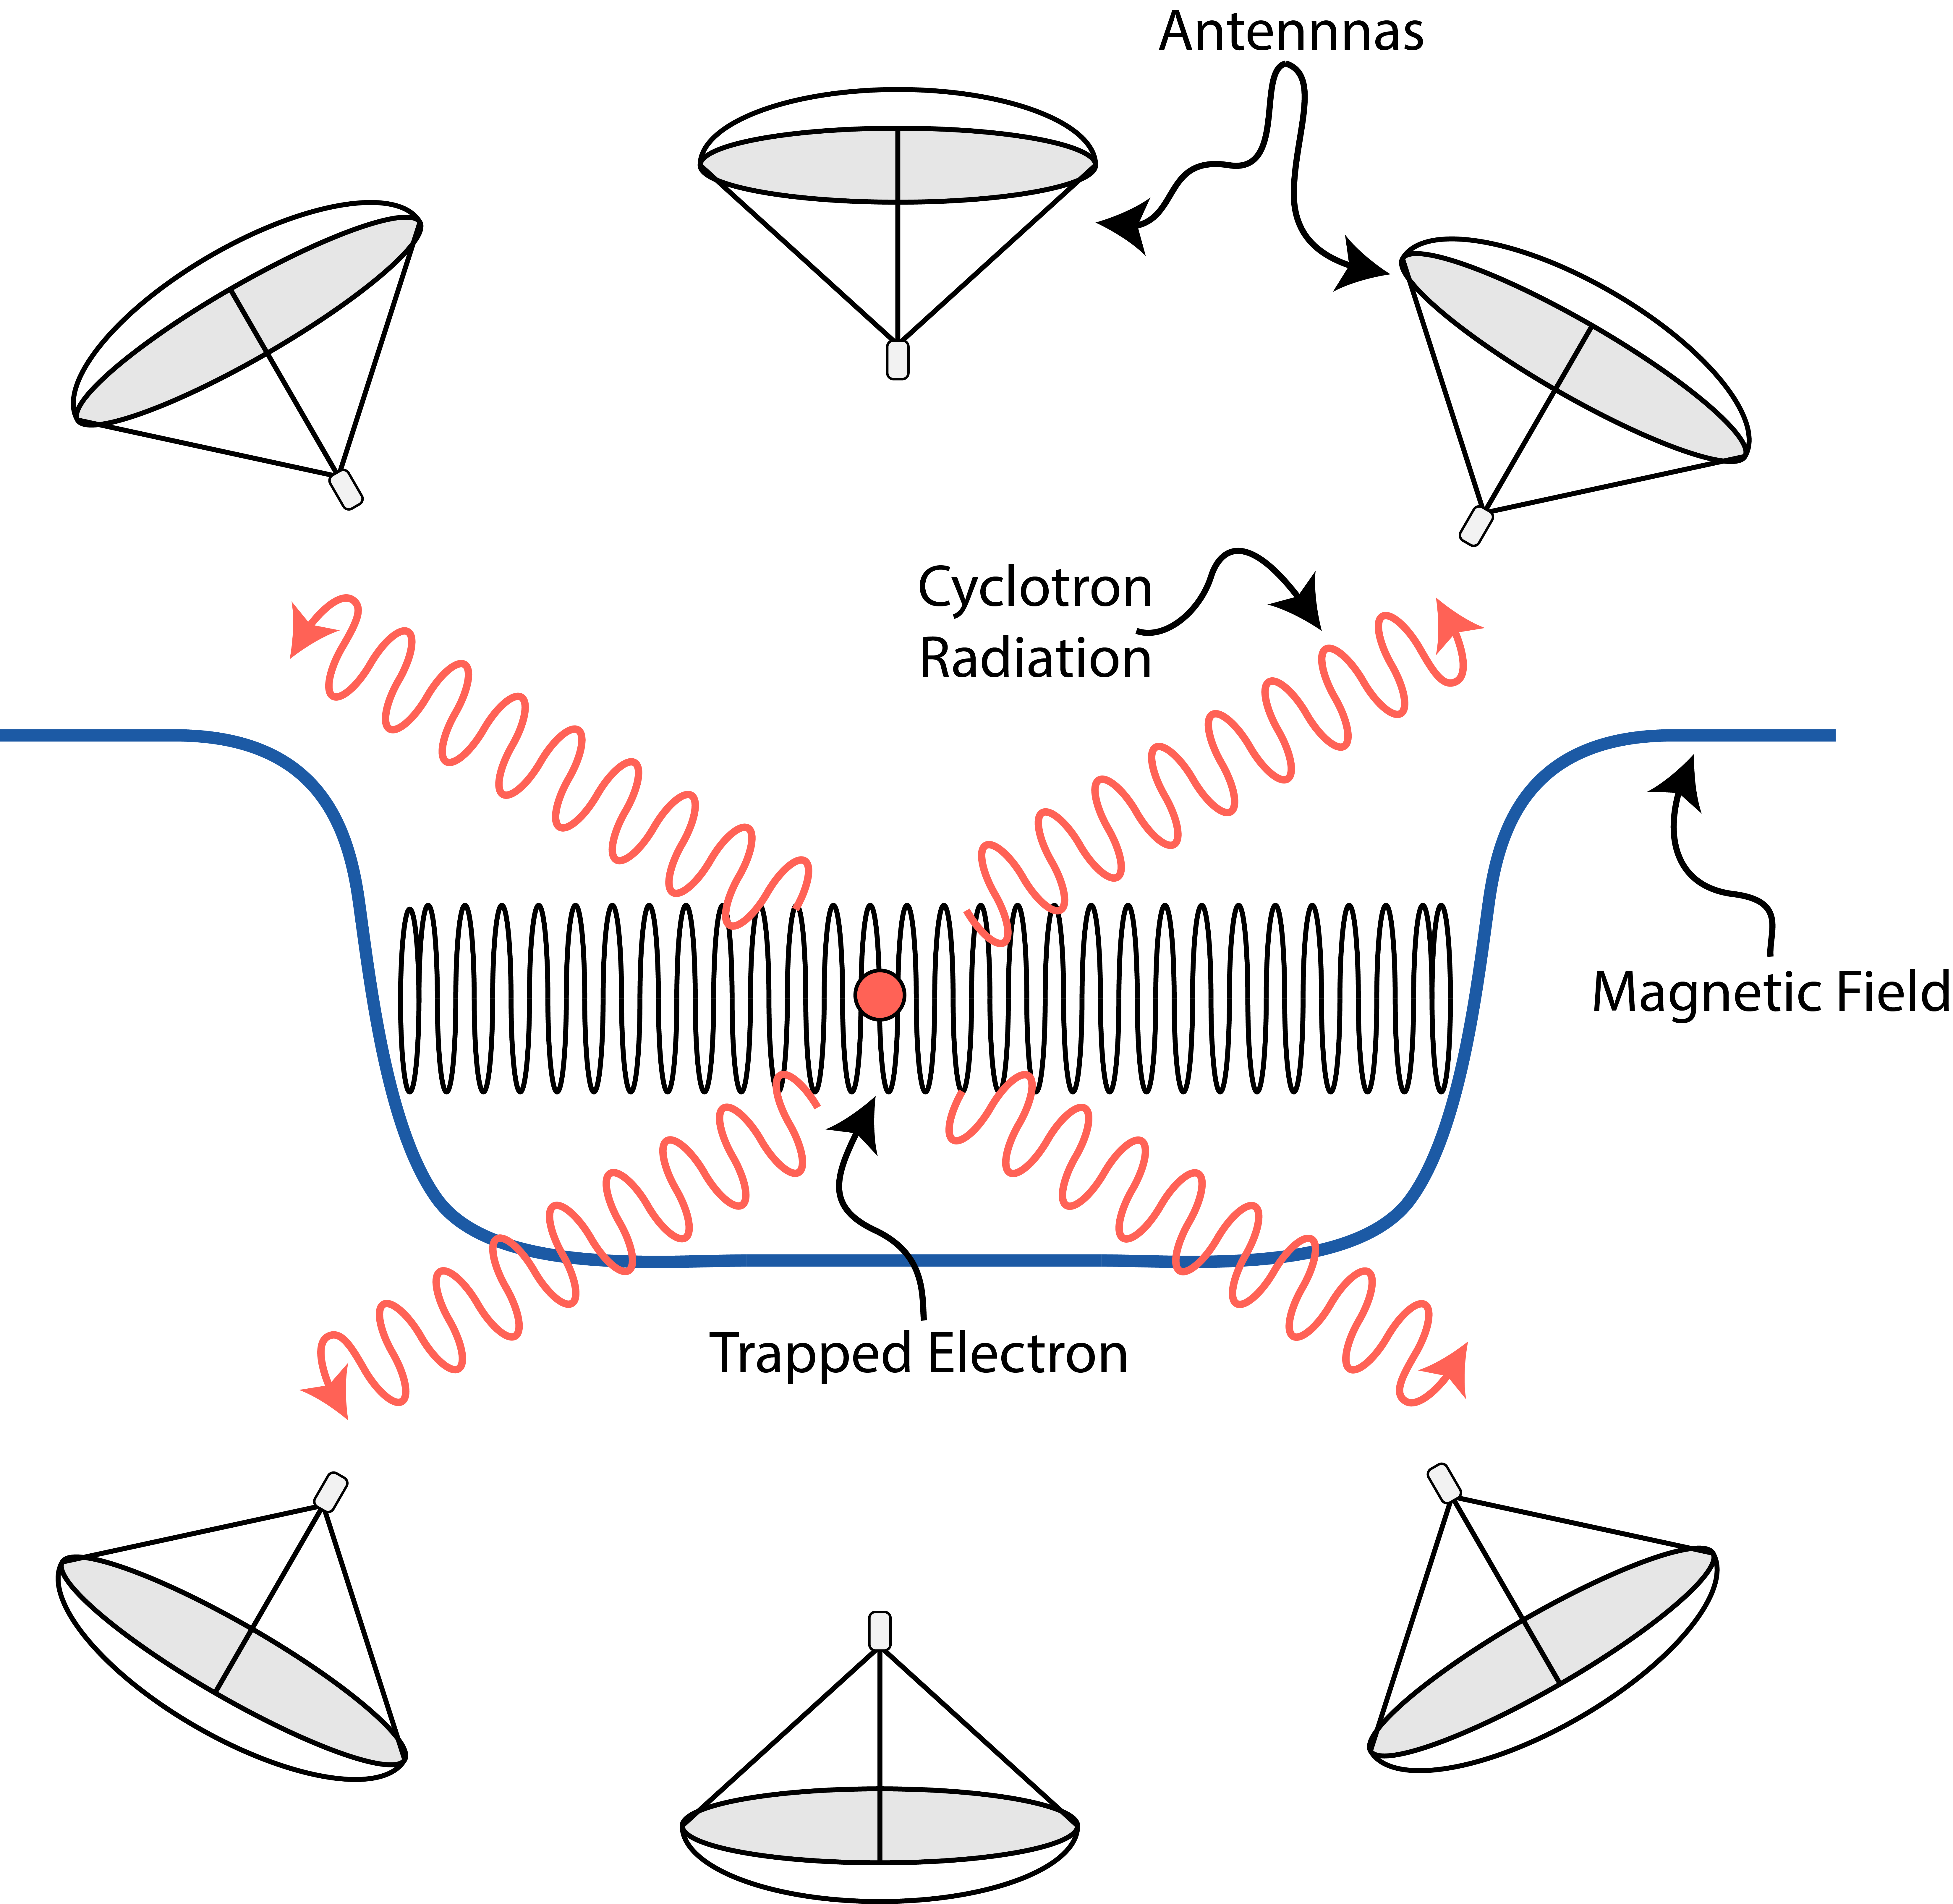
\includegraphics[width=0.5\textwidth]{figs/Chapter-3/230303_cres_cartoon.png}
    \caption{Caption}
    \label{fig:cres_cartoon}
\end{figure}

\subsection{Charged Particles in a Magnetic Trap}

\begin{figure}[htbp]
    \centering
    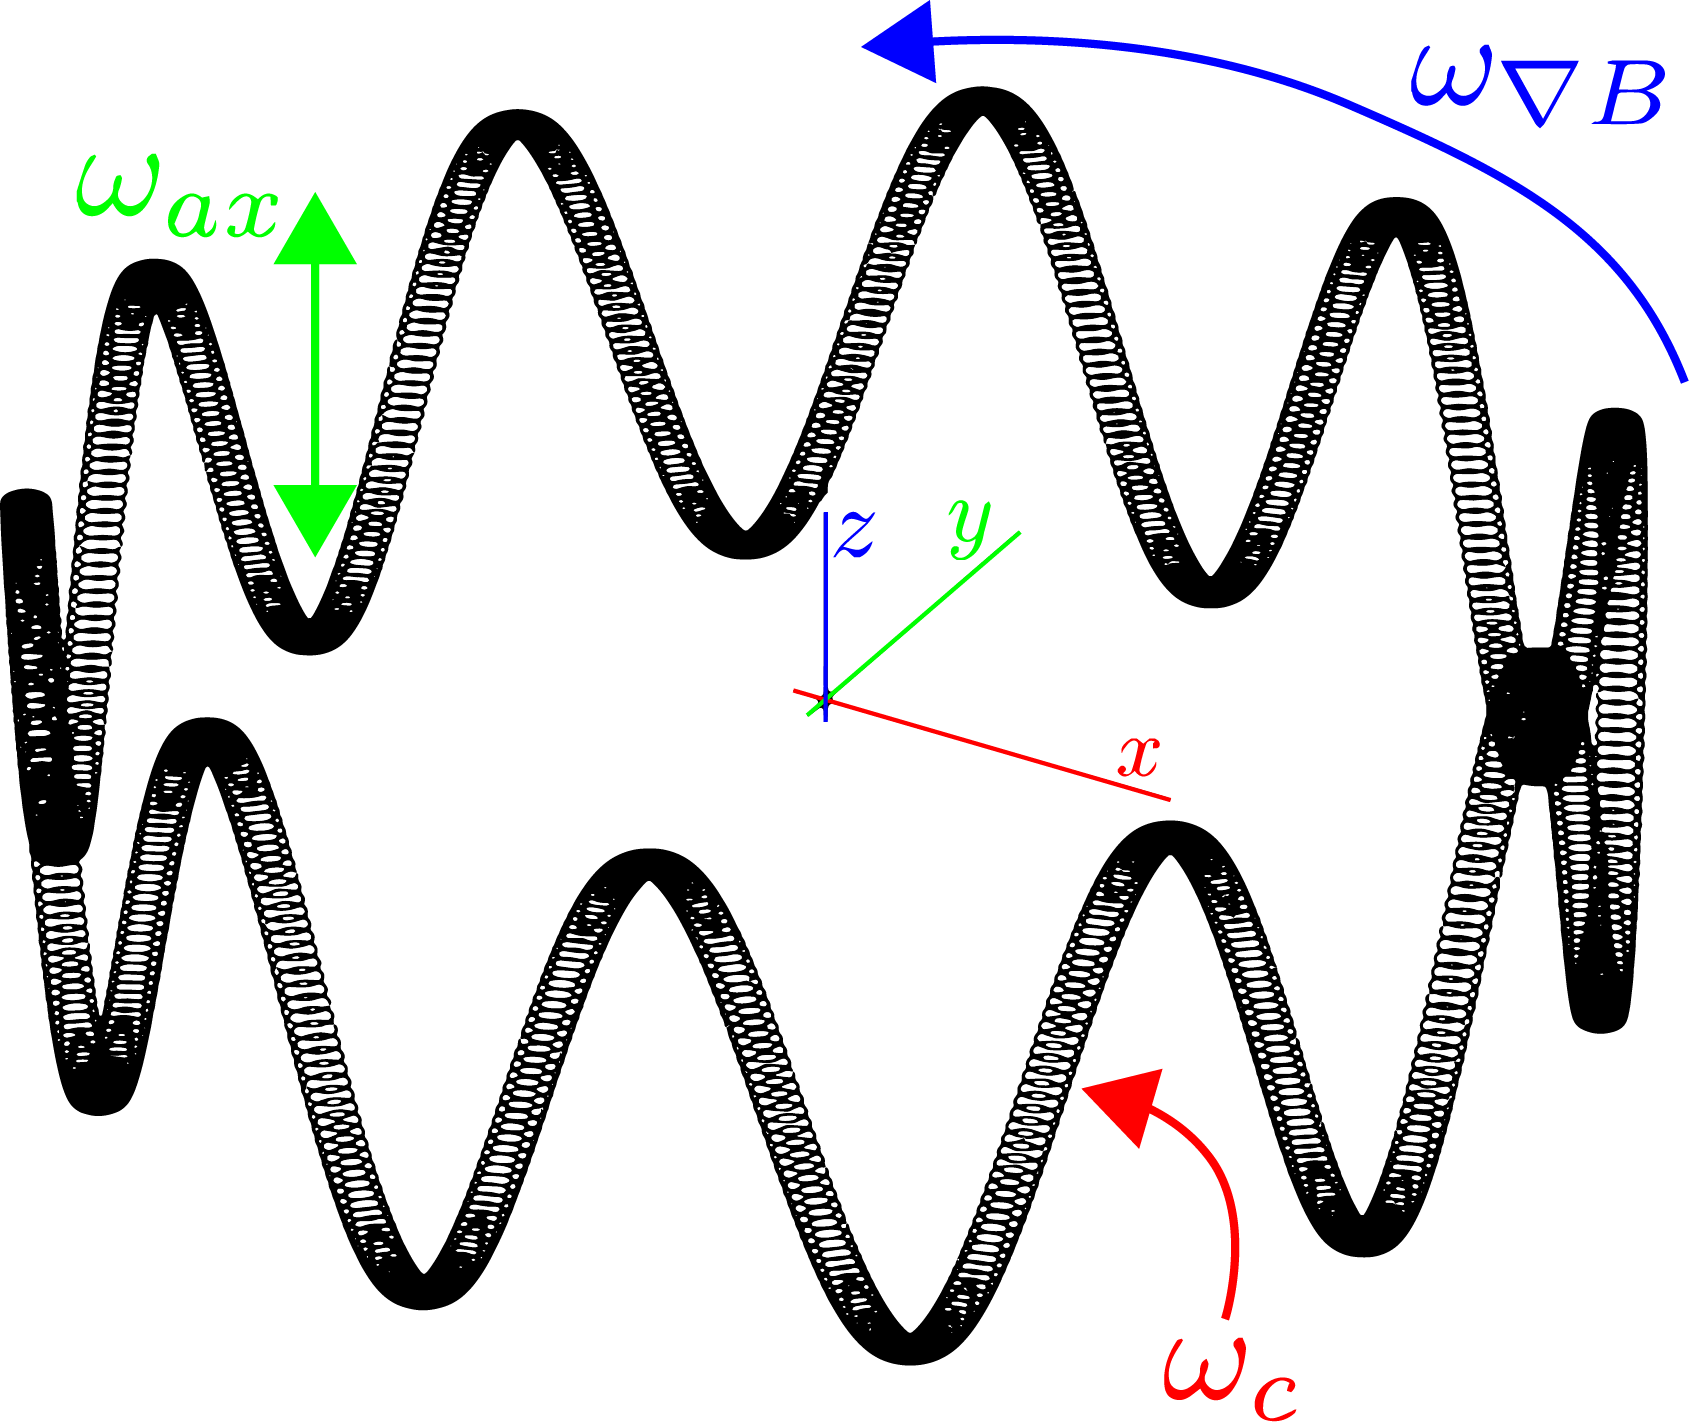
\includegraphics[width=0.5\textwidth]{figs/Chapter-3/230511_trapped_motion.png}
    \caption{Caption}
    \label{fig:chap3-trapped-electron-motion}
\end{figure}

\subsection{Radiation from a Charged Particle}

\section{The Project 8 Collaboration}

\subsection{Neutrino Mass Sensitivity Goals}

\subsection{Phased Development Plans}

\begin{figure}[htbp]
    \centering
    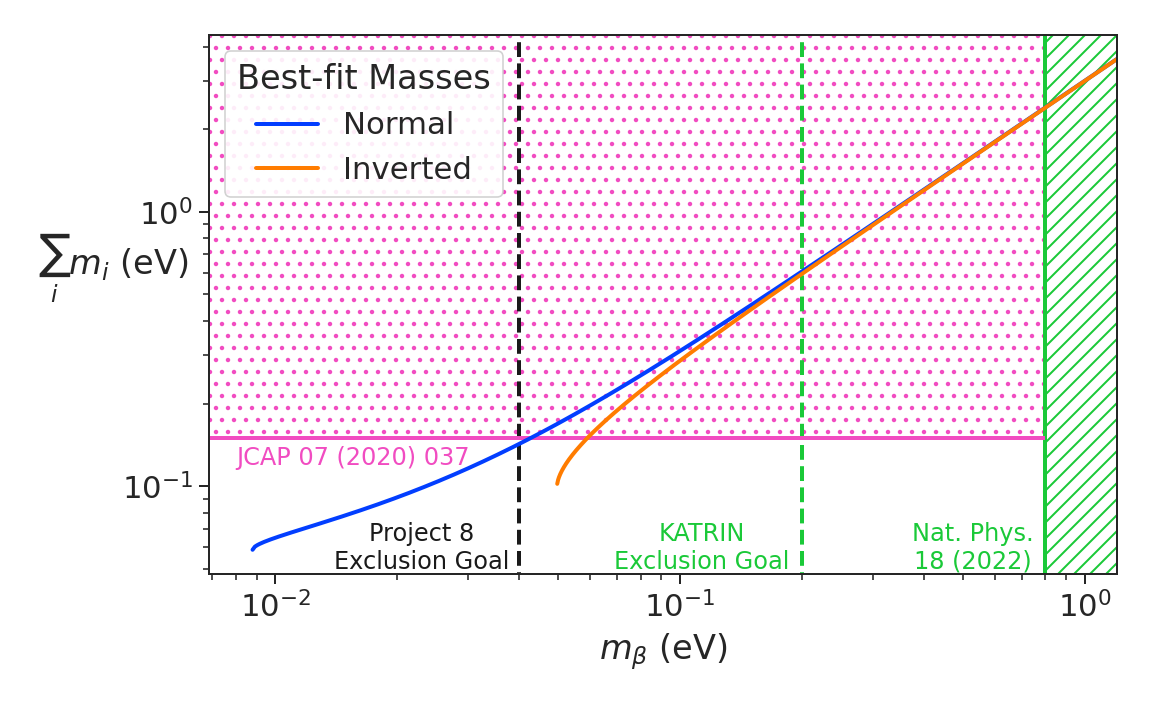
\includegraphics[width=0.7\textwidth]{figs/Chapter-3/230303_sum_nu_mass_vs_m_beta_with_exclusion_and_goal.png}
    \caption{Caption}
    \label{fig:p8_nu_mass_goal}
\end{figure}

\section{Phase II: First Tritium Beta Decay Spectrum and Neutrino Mass Measurement with CRES}

\subsection{The Project 8 CRES Demonstrator}

\begin{figure}[htbp]
    \centering
    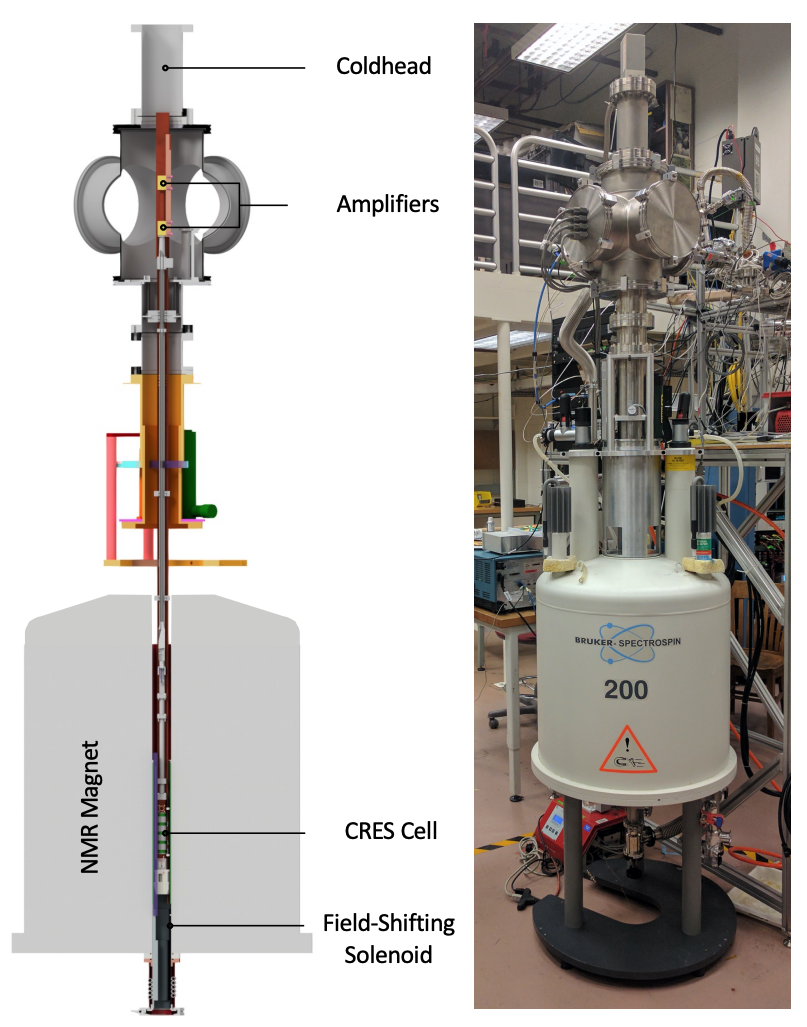
\includegraphics[width=0.7\textwidth]{figs/Chapter-3/phaseII_system.png}
    \caption{Caption}
    \label{fig:phase2_apparatus}
\end{figure}

\begin{figure}[htbp]
    \centering
    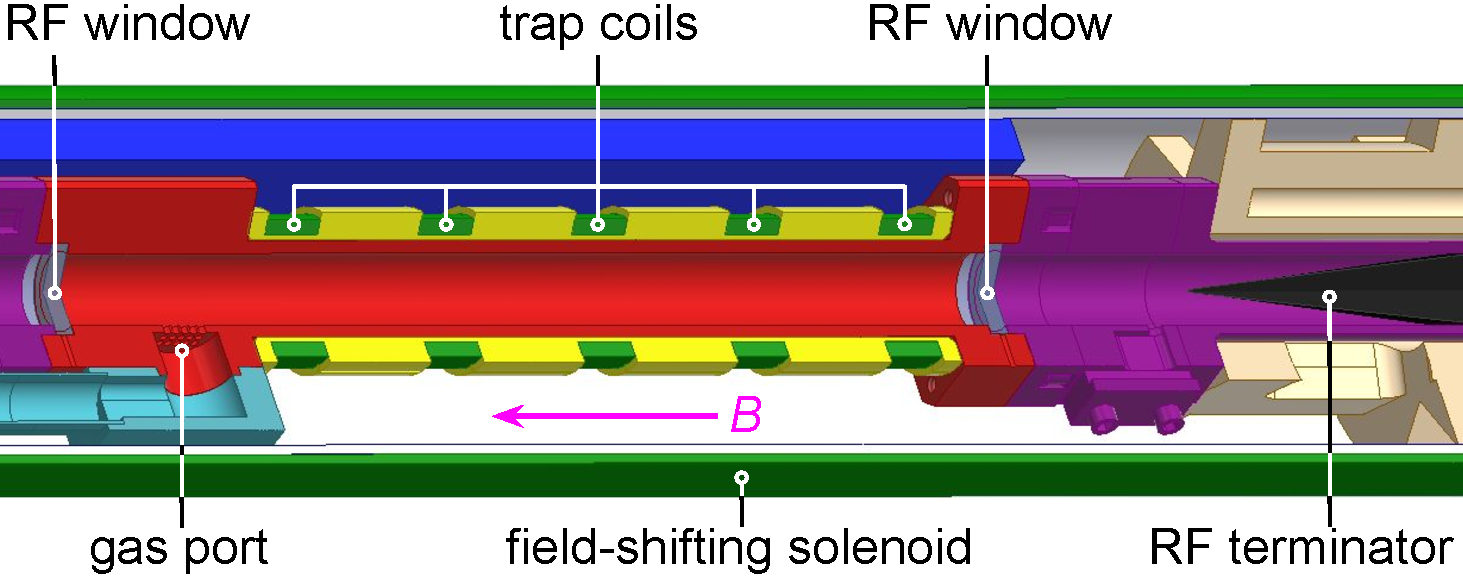
\includegraphics[width=0.8\textwidth]{figs/Chapter-3/apparatus.pdf}
    \caption{Caption}
    \label{fig:phase2_cres_cell}
\end{figure}

\subsection{CRES Track and Event Reconstruction}

\begin{figure}[htbp]
    \centering
    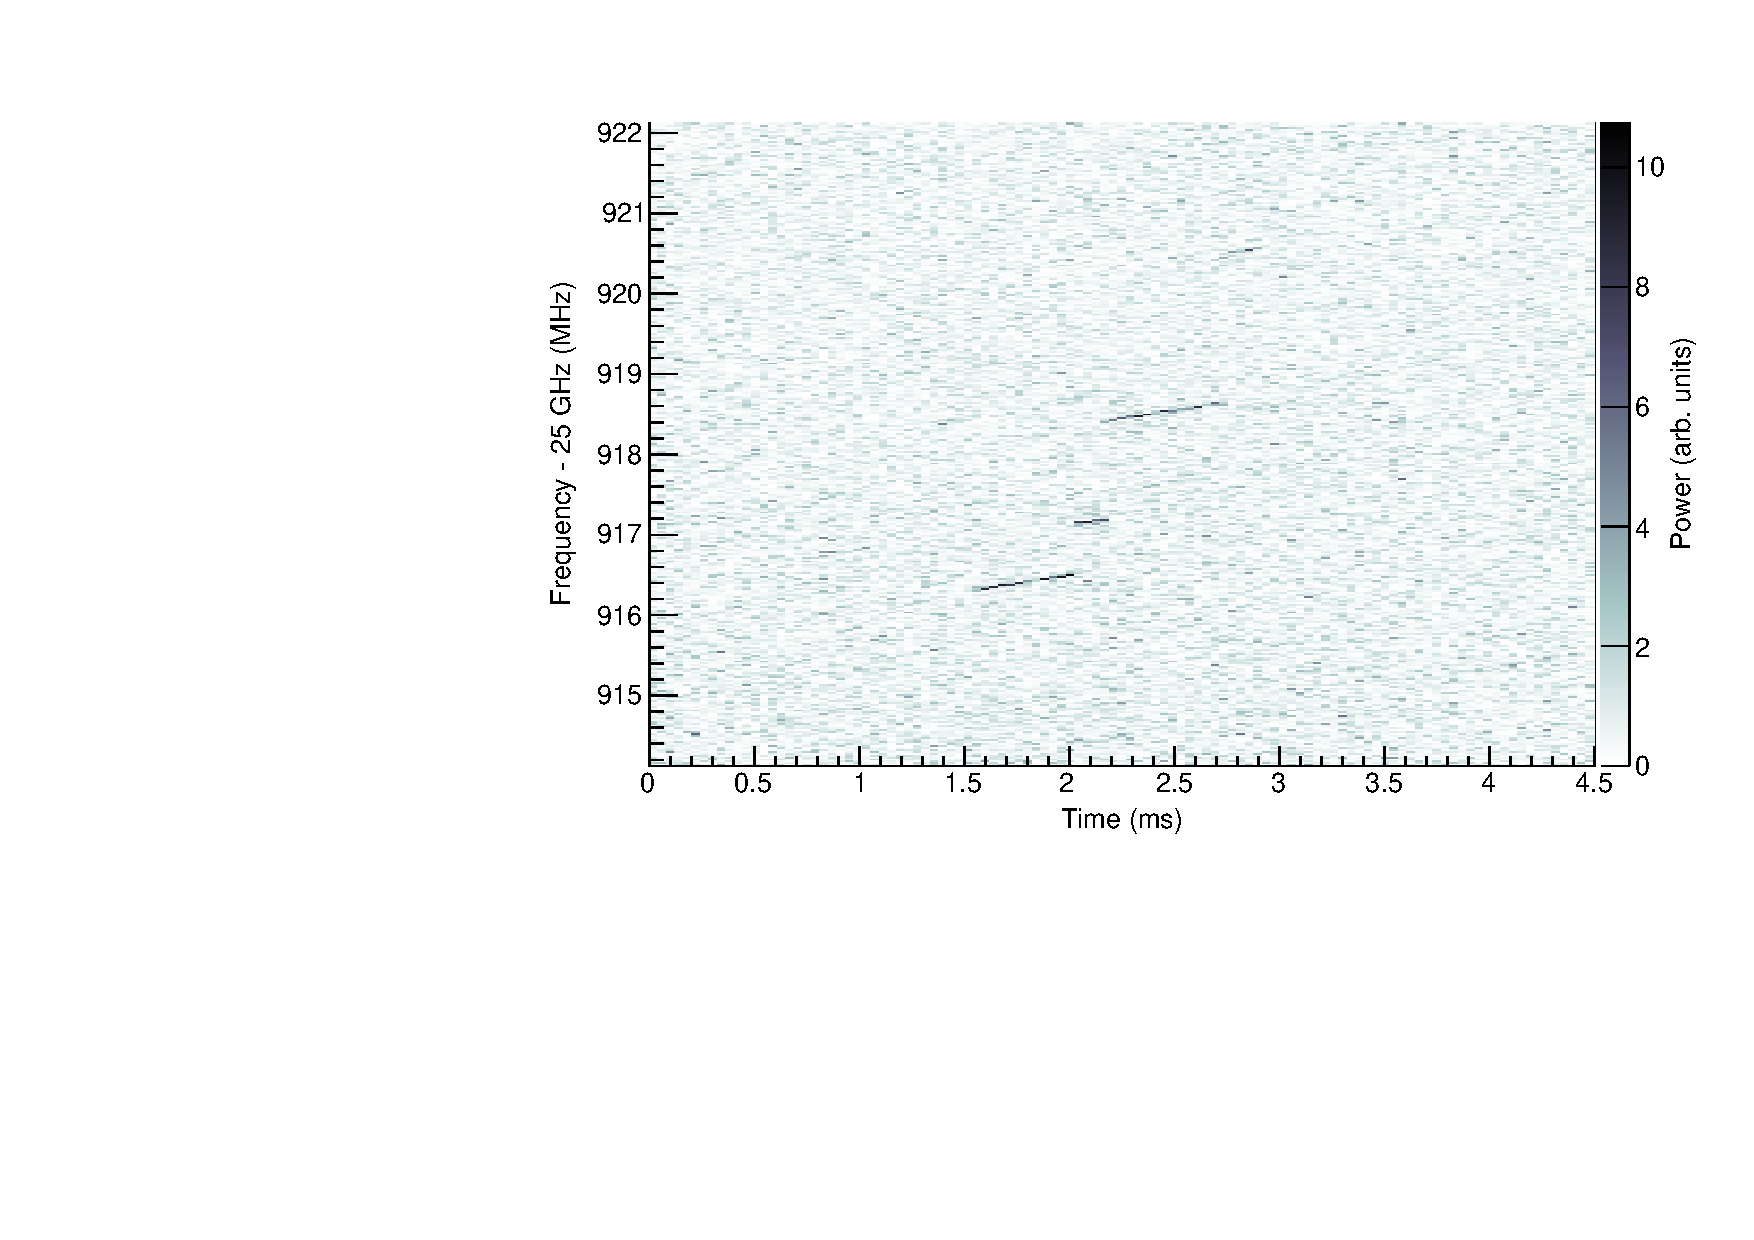
\includegraphics[width=0.7\textwidth]{figs/Chapter-3/T2_Event0.pdf}
    \caption{Caption}
    \label{fig:tritium_event0}
\end{figure}

\subsection{Measurements with Krypton}

\begin{figure}[htbp]
    \centering
    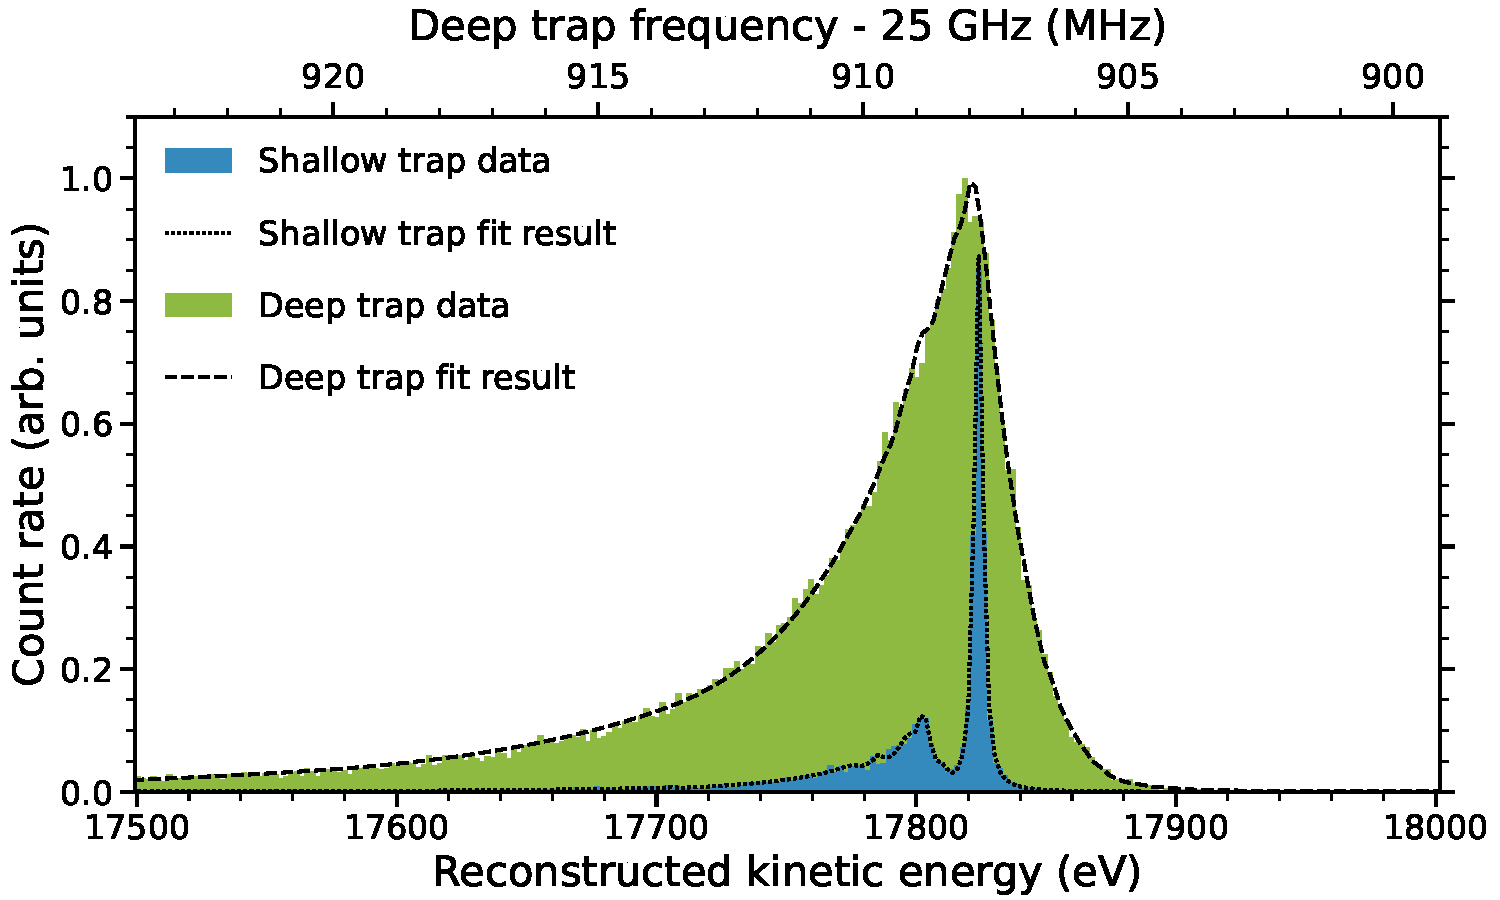
\includegraphics[width=0.7\textwidth]{figs/Chapter-3/kr_fit.pdf}
    \caption{Caption}
    \label{fig:krypton_fit}
\end{figure}

\begin{figure}[htbp]
    \centering
    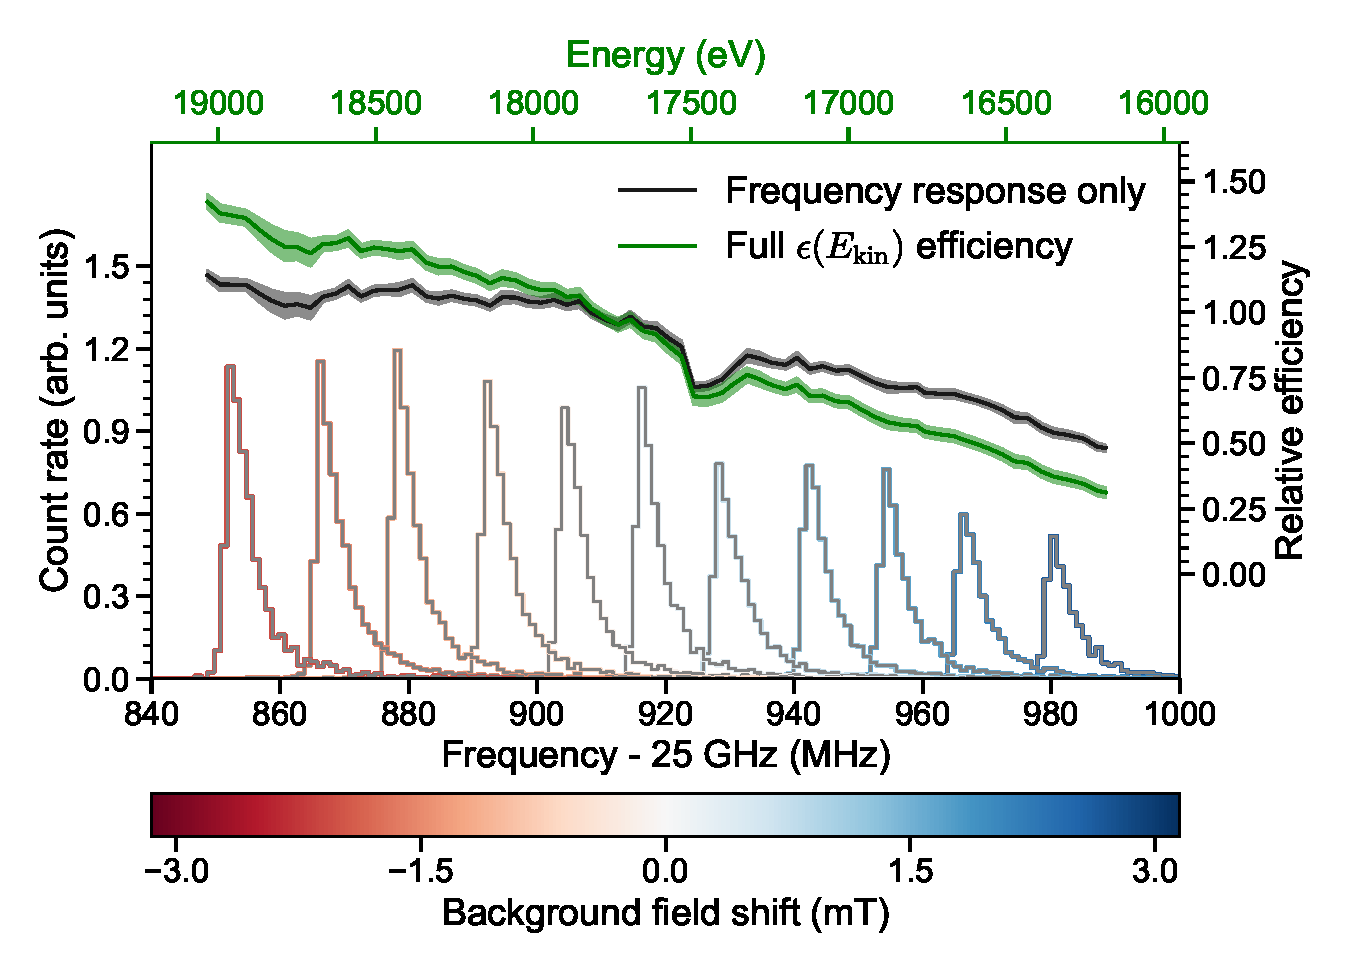
\includegraphics[width=0.7\textwidth]{figs/Chapter-3/fss_for_prl_plot.pdf}
    \caption{Caption}
    \label{fig:fss_plot}
\end{figure}

\subsection{Tritium Spectrum and Neutrino Mass Results}

\begin{figure}
    \centering
    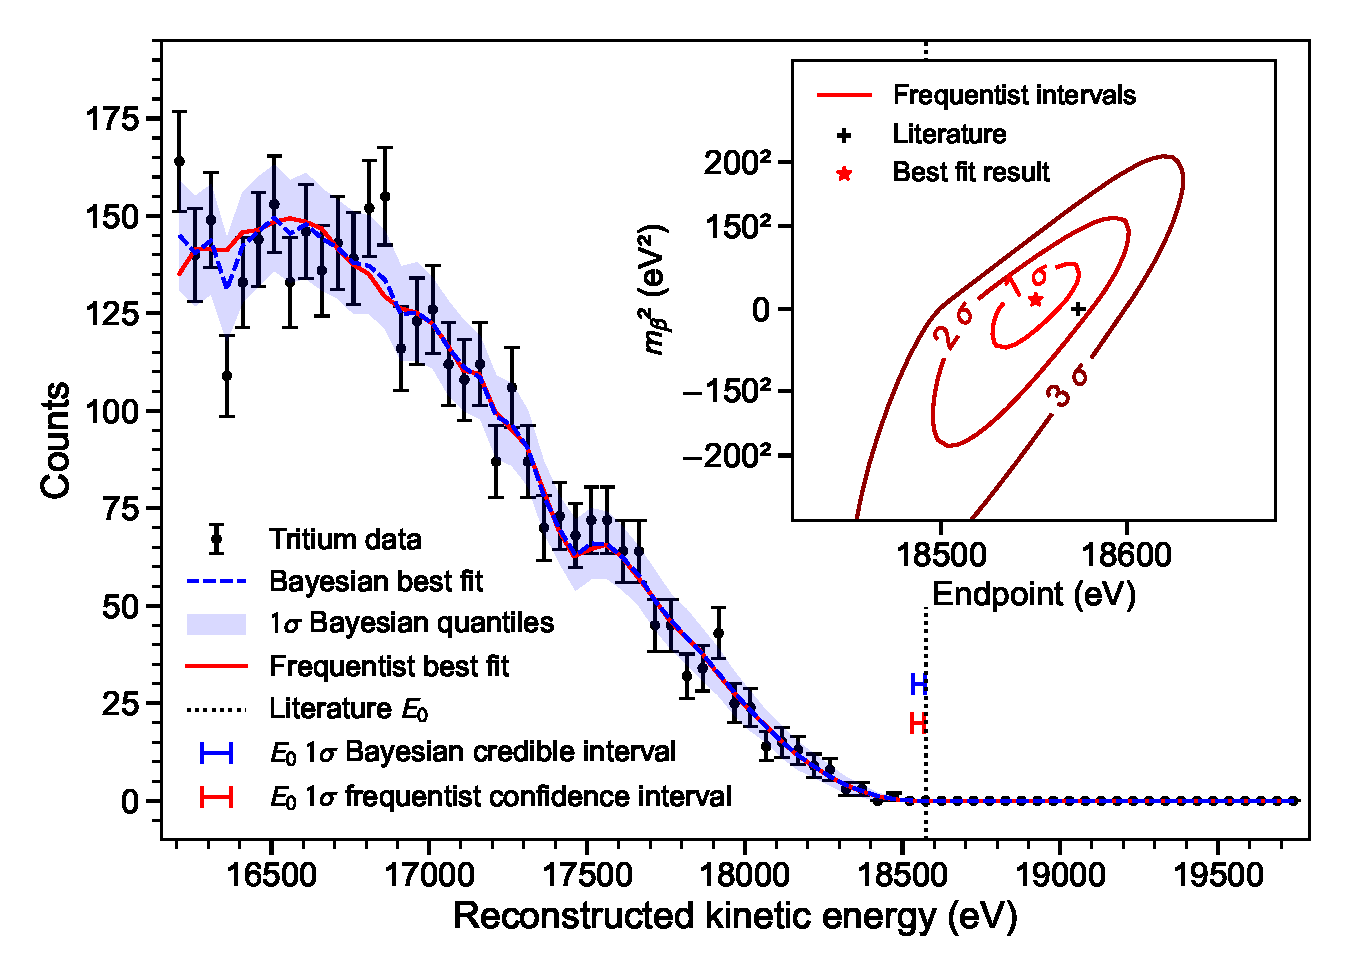
\includegraphics[width=0.7\textwidth]{figs/Chapter-3/12-03-22A_final_E0_real_data_phase_II_tritium_fit_1d.pdf}
    \caption{Caption}
    \label{fig:final_tritium_fit}
\end{figure}

\section{Phase III: Developing Free-space CRES Measurements with Antenna Arrays}

The goal of Phase III in the Project 8 experimental program is to develop the technologies and expertise required to build an experiment that uses CRES to measure the neutrino mass with a target sensitivity of 40~meV. One of the key technologies is a method for performing high resolution CRES measurements in a large volume, which allows one to observe a sufficient quantity of tritium to measure the low-activity endpoint region of the tritium spectrum. 

\subsection{The Basic Approach}

One possible approach, suggested in the original CRES publication, is to use many antennas to surround a volume of tritium gas in a magnetic field (see Figure \ref{fig:chap3-antenna-concept-cartoon}). When a decay occurs the electron will begin to emit cyclotron radiation that can be collected by the array and used to perform CRES.
\begin{figure}[htbp]
    \centering
    \includegraphics*[width=0.6\textwidth]{figs/Chapter-3/230614_antenna_cartoon.png}
    \caption{\label{fig:chap3-antenna-concept-cartoon}}
\end{figure}
Each antenna in the array collects only a small fraction of the electron's signal power, which is less than 1~fW for a 18.6~keV kinetic energy electron in a 1~T magnetic field. Scaling to large volumes with the antenna array approach is accomplished by increasing the number of antennas in the array, which increases the volume under observation proportionally, so that a sufficient population of tritium atoms can be observed to measure the tritium spectrum endpoint shape. 

Several features of the antenna array approach make it an attractive candidate technology for a large volume experiment. One example is the accurate position reconstruction made possible by the multichannel nature of the array. Using techniques like digital beamforming it is possible to estimate the radial and azimuthal positions of the electron in the magnetic trap with a precision significantly less than the size of the cyclotron wavelength. This capability allows one to perform event-by-event estimations of the magnetic field experienced by an electron, which is crucial to achieving high energy resolution with the CRES technique.

The easy availability of position information with the antennas array approach is potentially a unique advantage that provides significant flexibility in the magnetic field uniformity requirements compared to other proposed approaches to large volume CRES (see Chapter \ref{chap:cavity}). Spatial discrimination using digital beamforming leads to pileup reduction, which helps to reduce the potential of background events caused by missing tracks or by incorrectly clustering a group of tracks into an event. Limits on the background rate for a neutrino mass measurement with 40~meV sensitivity are stringent and the total activity of the tritium source for such an experiment is gigantic relative to the activity near the endpoint. Thus, pileup discrimination could be an important tool for a large scale CRES experiment.

Another beneficial quality of the antenna array approach is that the volume of the experiment can be scaled independent of frequency by simply adding more antennas to the array. Resonant cavities, the proposed alternative large volume CRES technology, are ideally operated in magnetic fields that cause electrons to move with cyclotron frequencies near the fundamental cavity resonance, to avoid complex coupling of the electron to many cavity modes simultaneously. This leads to a coupling between the cavity volume and the magnetic field magnitude, which forces one to lower the magnetic field in order to increase the experiment scale. Whereas, for antenna arrays, in principle there is no physical limitation on the size of the antenna array that can be used at a particular magnetic field. However, the nature of scaling an antenna array based experiment leads to rapidly increasing cost and complexity due to the large number of antennas, amplifiers, and data streams that require substantial computer processing power to effectively analyze.

\subsection{The FSCD: Free-space CRES Demonstrator}

The complex collection of new experimental techniques and methods that come together in the antenna array CRES technique require the construction of a small scale demonstration experiment designed to develop an understanding of the principles of antenna array CRES measurements and the relevant systematics. Without operating such an experiment it is not possible to develop a design for a large scale CRES experiment with sufficient confidence that the experiment is capable of measuring the shape of the tritium spectrum endpoint to the degree of accuracy required for 40~meV sensitivity to the neutrino mass. Therefore, Phase III of the Project 8 experimental program is primarily focused on the development and operation of demonstrator experiments to inform the design of the final Phase IV experiment.

Specifically for antenna array CRES, the associated demonstrator experiment in Phase III is called the Free-space CRES Demonstrator or FSCD. The goals of the FSCD include not only the development of antenna array CRES itself, but is also a capable neutrino mass measurement experiment in it's own right, with a target neutrino mass sensitivity of a few eV using a molecular tritium source.  

\subsubsection*{Magnetic Field}

The background magnetic field for the FSCD experiment is provided by a hospital-grade MRI magnet (see Figure \ref{fig:chap3-mri-magnet}). The magnet produces a magnetic field of approximately 0.958~T, which corresponds to a tritium spectrum endpoint frequency of approximately 25.86~GHz. 
\begin{figure}[htbp]
    \centering
    \includegraphics*[width=0.5\textwidth]{figs/Chapter-3/230614_mri_magnet.png}
    \caption{\label{fig:chap3-mri-magnet}}
\end{figure}
The magnet is installed in the Project 8 laboratory located at the University of Washington, Seattle, and is shimmed to produce a uniform magnetic field with variations on the ppm scale.

\subsubsection*{Antenna Array}

\begin{figure}[htbp]
    \centering
    \includegraphics*[width=0.4\textwidth]{figs/Chapter-3/230614_5slot_model.png}
    \caption{}
\end{figure}

\begin{figure}[htbp]
    \centering
    \includegraphics*[width=0.7\textwidth]{figs/Chapter-3/230614_fscd_render.png}
    \caption{}
\end{figure}

\subsubsection*{Gas System and Tritium Source}

\subsubsection*{Data Acquisition and Reconstruction}

\subsubsection*{Neutrino Mass Sensitivity}

\subsubsection*{Scaling}

\begin{figure}[htbp]
    \centering
    \includegraphics*[width=1\textwidth]{figs/Chapter-3/phaseiv_concept_sketch_ver2.png}
    \caption{}
\end{figure}


